\documentclass[review]{elsarticle}

\usepackage{lineno,hyperref}
\modulolinenumbers[5]

\usepackage{pgfplots}

\journal{Journal of \LaTeX\ Templates}

%%%%%%%%%%%%%%%%%%%%%%%
%% Elsevier bibliography styles
%%%%%%%%%%%%%%%%%%%%%%%
%% To change the style, put a % in front of the second line of the current style and
%% remove the % from the second line of the style you would like to use.
%%%%%%%%%%%%%%%%%%%%%%%

%% Numbered
%\bibliographystyle{model1-num-names}

%% Numbered without titles
%\bibliographystyle{model1a-num-names}

%% Harvard
%\bibliographystyle{model2-names.bst}\biboptions{authoryear}

%% Vancouver numbered
%\usepackage{numcompress}\bibliographystyle{model3-num-names}

%% Vancouver name/year
%\usepackage{numcompress}\bibliographystyle{model4-names}\biboptions{authoryear}

%% APA style
%\bibliographystyle{model5-names}\biboptions{authoryear}

%% AMA style
%\usepackage{numcompress}\bibliographystyle{model6-num-names}

%% `Elsevier LaTeX' style
\bibliographystyle{elsarticle-num}
%%%%%%%%%%%%%%%%%%%%%%%

%% Custom commands:
\newcommand{\model}{\textbf{\textit{MountGrass}}~}



\def \slope{2}

%%%%%%%%%%%%%%%%%%%%%%%

\begin{document}

\begin{frontmatter}

\title{General framework for coexistence including phenotypic plasticity: the model \model}
\title{The individual basis of plant coexistence in mountain grassland and the effect of phenotypic plasticity: investigation with the model \model}
\tnotetext[mytitlenote]{Fully documented templates are available in the elsarticle package on \href{http://www.ctan.org/tex-archive/macros/latex/contrib/elsarticle}{CTAN}.}

%% Group authors per affiliation:
\author{Elsevier\fnref{myfootnote}}
\address{Radarweg 29, Amsterdam}
\fntext[myfootnote]{Since 1880.}

%% or include affiliations in footnotes:
\author[clement.viguier@irstea.fr,mysecondaryaddress]{Clément Viguier}
\ead[url]{www.elsevier.com}

\author[mysecondaryaddress]{Global Customer Service\corref{mycorrespondingauthor}}
\cortext[mycorrespondingauthor]{Corresponding author}
\ead{support@elsevier.com}

\address[mymainaddress]{1600 John F Kennedy Boulevard, Philadelphia}
\address[mysecondaryaddress]{360 Park Avenue South, New York}

\begin{abstract}
\end{abstract}

\begin{keyword}
\texttt{elsarticle.cls}\sep \LaTeX\sep Elsevier \sep template
\MSC[2010] 00-01\sep  99-00
\end{keyword}

\end{frontmatter}

\linenumbers

\section{Introduction}

Global change has been subject of a large, and still growing, number of studies. Yet, because the complexitiy of ecological system coupled with the uncertainty around the future of climate and management, a lot of work is remaining to predict the state of natural and semi-natural systems in the future. Vegetation communities are of particular interest as they provide both economic value and ecosystem services. If a large part of plant community ecology is foccused on forests, the presumed vulnerability to global change of mountain grasslands has led scientists to study them. If their actual vulnerability is still discussed (phd of sandra, ecoveg 2015), mountain grasslands will certainly be exposed to increasing temperature and droughts, but also to changes in management practices with a reduction of grazing (ask greg, see ref in ceres baros first paper).\\
To better understand and predict the effect of global change in these ecosystems of mountain grasslands, empiricall studies and experiments have been set. (see Jena, leca and Levine). These studies and others (Violle, albert, jung) highlight the importance of intra-specific variations in community ecology. Intra-specific variations represent around 20 and 30 percent of total variation in grasslands (see albert) and could greatly alter the species interactions and community response to abiotic factors. Considering intra-specific variations is important to better understand community dynamics (violle) and in models because they favour coexistence (Clark, Jung, Courbaud) and modify community responses (Jung). Such effects are succeptible to greatly influence the dynamic of communities facing global change by mitigating species level response, soften plant niches frontier, altering species competition. Another argument is the fact that intra-specific changes may alter directly the community response to a stress (Jung).\\

 Moreover the role of long term evolutionary and ecological processes cannot be easilly assessed in such designs. Moreover, considering the multiplicity of climatic and management scenarios scales up the work to a limiting point.\\



To overcome these limitations and difficulties, modelling approaches has been developped (fate-h, samsara, taubert, lohier ...). They are either used for the retrospective studies long term dynamics from time series data, the prediction of community dynamics along different scenarios, or to interogate the underlying mecanisms of community dynamics (gemini). These models, to be able to account for changing condittions are all based on strong plant functioning processes at the scale of interest and are supported by field data through parametrisation.\\


Most of these models feature a fixed plant functioning where the dynamic of the community is mostly driven by, 1) the abiotic conditions, 2) the relative competitiveness of species/group specific parameters or direct competion coefficients. If 1) is essential in the context of climate change, the point 2) as main mechanism of plant interaction can be discussed as it relies on differences between species specific physiological parameters. Physiological or competition parameters are generally estimated by direct measures or derived from dta through calibration. Both methods give estimators in what we have good confidence, however they do not allow them to vary within the group (plant functional type, species or population) they have been defined for. The estimator produce good results and generally follow fundamental or ecological trade-offs. Yet, they do not allow for variations within the group for these parameters, as they are not strictly constraint by said trade-offs and could lead to Darwinian demons, or would require calibration of this variation space. More efforts must be done in the representation of the link  between chemical, anatomical and morphological traits and physiological traits that drive plant growth and plant interactions. Defining such link would authorise variations within a group while maintaining strong trade-offs between physiological traits and allowing variation and search in the strategy space... (not clear).\\

We stressed the importance of considering intra-specific variations, ann highlight the necessity for a link between chemical and anatomical traits to functioning traits.  
 Not clear what is genetic variation and selection/evolutionary processes or phenotypic plasticity. Phenotypic plasticity in models: theoretical: 2 species interactions, not at community model. (Heritability ?)




There is a need for community models capable of reproducing diverse plant communities. To investigate the effect of climate change it has to incorporate mechanism of response and individual level.\\
Such mechanism is called phenotypic plasticity\\

\textbf{
How is it really different from source-sink approaches ? Or functional equilibrium ?}
-> allocation based, trait variations, plasticity is a strategy. This last poinnt is important. It's related to the discussion around van kleunen ad Dewitt (not all species are plastic, sultan says most are) <- check that.\\

The need of mechanistic model integrating functional traits and carbon allocation ... \cite{marechaux_individual-based_2017} + probably general reviews on vegetation modelling

\section{Methods}
\subsection{Model overview and concepts}
\paragraph{Overview of \textit{MountGrass}}
\paragraph{Plasticity in \textit{MountGrass}:
 concepts and implementation}

\textbf{Allocation} Why allocation and not just traits ? Allocation model provide structural constraint for plant strategies. Study ecology is studying the relative performance of individuals (and their impact on environmental conditions) in relationship with their strategies. Considering the amount of traits and strategies plants can develop, it is crucial to reduce the dimensionality of the strategic space (space define by all independent strategic axis plant can be found on). The most effective way to use laws of physics, chemistry and biology to eliminate impossible strategies (or combination of traits). Allocation based model take advantage of the "law of mass balance" ... to limit the number of possible allocation pattern, or strategies. This approach has the advantage of creating limited \textit{continuous} strategy space that can be explored and reveal ecological relationships/constraint. The search for such relationships or trade-offs is a big challenge in empirical ecology (see \cite{reich_evolution_2003, wright_worldwide_2004, diaz_plant_2004, diaz_global_2016} for plants) and ecological modelling (see \cite{reineking_environmental_2006, falster_plant:_2016}) as they reduce the complexity and help understand the main mechanisms that shape communities.\\
Introduce the idea of default strategy with this ratio of active vs structural tissues.


\textbf{Plasticity}: expected environment -> phenotype, here phneotype is equivalent to biomass partitioning, that means expected environement -> allocation coefficients. Then memory -> expectations -> allocation. Because low dimensions, and we want diversity, and the link between memory and allocation might not be a function (one memroy give exactly one optimum allocation), in the model this relationship is not verified. Species specfic traits are used to allow for different strategies to be associated to a same memory (different plants won't have the same strat, despite sharing the projection)\\
Once the plasticity is introduced, talk about the memory. Now you can also talk about the mapping/consistency between both and the difficulties to use both.

\textbf{Allocation algorithms}


\subsection{Calibration}
\paragraph{Pot data}
Pot data consists in total biomass and root shoot ration (RSR) data of ... species grown in pots by Peterson and al. (peterson). This old dataset has the advantages of being grass species grown in a described steady environment with two conditions of watering with measures of essential components of growth: biomass and RSR. The inputs used to simulated these experriment are detailed in appendix.

\paragraph{Individual calibration process}
Bayessian calibration could not be used for the model considering the number of parameters and the simulation time. A filtering process has been implemented in R. Parameters are sampled following the LHS method (from \texttt{lhs} package)	within parameter ranges (desccribed in table ...) defined from the litterature, and constraints dicted by desired behaviours from the model. When necessary the sample is log transformed. Because of strong relationship between exchange rate parameters and cost of exchagne area, exchanges rates parameters are expressed on a mass basis for sampling then transform to an area basis for the model. Phtosynthetic activity is defined relatively to the water uptake activity and water use efficiency (WUE) to avoid extreme root shoot ratios.\\

Once generated a first filtering is applied to save simulation time and avoid unrealistic trait values (see table for ranges extracted from LES data in alpine biome) that are not tested against calibartion data.\\
Once the parameters transformed and filtered, simulations matching growth conditions in Peterson experiments.\\
Generated data from finished simulations (i.e. plant lives until the end and do not exceed model's internal size limits) are then compared to experiment data species by species. Parameters of logistic distribution are computed from species means and standards deviantions for RSR and total biomass. The use of this distribution form is justified by the intrinsic form of RSR measure and the need to reject negative values for total biomass. A parameter set is accepted for one species if it within a 95\% range of the calculated distribution for both RSR and total biomass in wet and dry conditions.\\

\paragraph{Strategy diversity filtering}
To further reduce the number of parameter sets considered, we proceeded in an additional filtering step. Because the first filtering was conduced for only one strategy over the whole 4D strategy space (l\_ini,  w\_ini, as\_s\_d, as\_r\_d) it is necessary to verify that other strategies do not lead to potential Darwinian demon. This should be limited by the choice of priors, while at the same time promoted by the selection of parameters increasing growth to counter balance potential unfitted strategies\footnote{Better do that beforehand than after... But I guess it's too late now.}.

\paragraph{Field calibration}
New random parameters sets (with no species specific parameters) for population dynamics and competition specific parameters (see table ...).
Sequence of around 60 year for each site. Parameters were selected by...


\paragraph{Field data}
Field data has been collected between years 201 .. and 201 by Claire Deleglise and al. ().

\paragraph{Weather data}
Weather data has be computed by the MeteoFrance model SAFRAN by ... using GPS coordinates and slope, azimuth and horizon computed from a "MNT". These parameters were also used by the model CROCUS to compute snow accumulation and melting. These high frequency data (resolution under 1h) have been average daily and used to compute input variables for \model . 

\subsection{Simulation setup}
All common parameters for pot simulations. i.e. weather, soil, default species parameters.



\section{Results}
\subsection{Growth of diverse species}
\paragraph{Individual calibration}. Calibration filtering results in the selection of n parameter sets over m preselected parameters sets. Accepted sets are distributed among the 11 species of the dataset like presented in the table. Species A, B and C are the most numerous.\\
sensitivity analysis. The models about seems to be sensitive to the following parameters: $r_1$, $\beta_0$, $P_{max}$, $u_{max}$, $k_{or}$, $\rho_{ar}$. The four first parameters are related to global resource availability and directly related to growth rate, while the second and the last three and related to the below-ground resource foraging and exchange rate.\\
Total biomass is particularly sensitive to exchange rate parameters, but also tissue construction cost. (not shown)\\

Plasticity does not change the acceptance rate in any form (only slight increased from 0.26\% to 0.38\%). Despite non overlapping (around respectively and third and a quarter of accepted parameter sets are shared between non plastic and plastic calibration) the distribution of not shared parameter sets are very similar and does not show any clear pattern. \\

\begin{figure}
\includegraphics[width = \textwidth]{/mnt/quadri1/simulations/exploration/species_par_space2017-10-26/plots/acceptance_rate_RSRnWeight_per_par.pdf}
\caption{Acceptance rate per parameter for individual growth. No plasticity}
\end{figure}

\begin{figure}
\includegraphics[width = \textwidth]{/mnt/quadri1/simulations/exploration/species_par_space2017-11-06/plots/acceptance_rate_RSRnWeight_per_par.pdf}
\caption{Acceptance rate per parameter for individual growth. RSR plasticity}
\end{figure}

Acceptance rate without plasticity:
% latex table generated in R 3.2.3 by xtable 1.8-2 package
% Wed Nov 15 13:36:59 2017
\begin{table}[ht]
\centering
\begin{tabular}{rlrr}
  \hline
 & species & nb accepted & rate \\ 
  \hline
1 & Silene acaulis & 227 & 0.02 \\ 
  2 & Trifolium dasyphyllum & 271 & 0.03 \\ 
  3 & Geum rossii & 51 & 0.01 \\ 
  4 & Thlaspi alpestre & 342 & 0.03 \\ 
  5 & Deschampsia caespitosa & 0 & 0.00 \\ 
  6 & Eriogonum umbellatum & 500 & 0.05 \\ 
  7 & Townsendia scapigera & 593 & 0.06 \\ 
  8 & Astragalus whitneyi & 1570 & 0.16 \\ 
  9 & Lupinus lobbii & 678 & 0.07 \\ 
  10 & Erigeron peregrinus & 1 & 0.00 \\ 
  11 & Oxyria digyna & 0 & 0.00 \\ 
   \hline
\end{tabular}
\end{table}

Acceptance rate with RSR plasticity for equilibrium:
% latex table generated in R 3.2.3 by xtable 1.8-2 package
% Wed Nov 15 13:39:16 2017
\begin{table}[ht]
\centering
\begin{tabular}{rlrr}
  \hline
 & species & nb accepted & rate \\ 
  \hline
1 & Silene acaulis & 396 & 0.04 \\ 
  2 & Trifolium dasyphyllum & 317 & 0.03 \\ 
  3 & Geum rossii & 72 & 0.01 \\ 
  4 & Thlaspi alpestre & 360 & 0.04 \\ 
  5 & Deschampsia caespitosa & 0 & 0.00 \\ 
  6 & Eriogonum umbellatum & 805 & 0.08 \\ 
  7 & Townsendia scapigera & 930 & 0.09 \\ 
  8 & Astragalus whitneyi & 2424 & 0.24 \\ 
  9 & Lupinus lobbii & 868 & 0.09 \\ 
  10 & Erigeron peregrinus & 0 & 0.00 \\ 
  11 & Oxyria digyna & 0 & 0.00 \\ 
   \hline
\end{tabular}
\end{table}


Change of relationship between parameters and acceptance rate -> none\\
accept = f(tau)\\

PCA reveal that sensitive parameters are also the dominant variables in the main components of the component analysis of the accepted parameter sets. Species cannot be distinguished on the two main component space, neither on 1 or 2D species specific parameters space (l\_ini, w\_ini, w\_ini vs l\_ini, as\_s\_d, as\_r\_d, as\_r\_d vs as\_s\_d) despite small variations in distribution shapes between species.\\



\begin{figure}
\includegraphics[width = 10cm]{/mnt/quadri1/simulations/exploration/species_par_space2017-11-06/plots/var_imp_plot_eq_design.pdf}
\caption{Importance of the random forest to explain filtering outcome (accepted or rejected) of a balanced sample of parameter set between all tested (all accepted parameters and an equivalent sample in rejected parameters).  RSR plasticity.}
\end{figure}

\begin{figure}
\includegraphics[width = 10cm]{/mnt/quadri1/simulations/exploration/species_par_space2017-11-06/plots/PCA_acc.pdf}
\caption{Accepted parameters set for plastic individual growth calibration filtering  on the two main components of PCA.}
\end{figure}

\paragraph{Individual growth pattern and plasticity}

Individual growth and allocation looks like that:\\
change in size of different pools (shoot, active, shoot str, stem ..., rep, storage). Plus constant traits.\\

Different allocation algorithms change the growth but also the traits:\\
BMtot, RSR, SRL and SLA of the same plant with different algorithms, other things being equal.

\begin{figure}
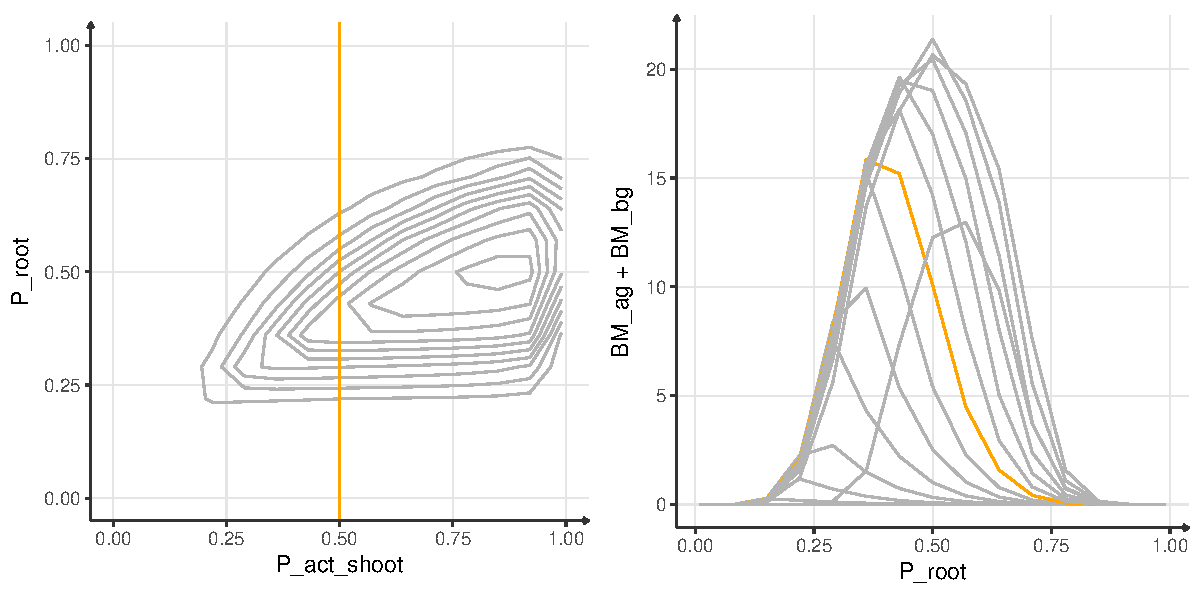
\includegraphics[width = \textwidth]{./Figures/Perf_landscape.pdf}
\caption{Performance landscape.}
Landscape accessible with only RSR plasticity. Part of the landscape (especailly) optimum is not accessible without trait plasticity.
\end{figure}

\paragraph{Active versus structural: the foundation of the niche}

Niche results from the absolute (potential niche) or relative (realised niche) performance of individual plant along environmental gradient. Performance (if measured as living biomass at a given time) in \model is a composite variable depending on: the absolute efficiency of the different organs (shoot and root), the relative proportion of these organs, and the equilibrium between shoot and root activity.\\
Theoretical performance trade-off: result from the mathematical expression of construction cost of tissue and their exchange rates.\\

\textit{figure and formulas}
\begin{figure}
\begin{tikzpicture}
\begin{axis}[
legend style
={at={(1, 1.1)},
anchor=south east,
draw = none},
samples = 100,
%restrict y to domain=-300:700,
xlabel = $\theta$,
ylabel = $U_{lim}$
%extra x ticks={0.618},
%extra x tick style={grid=major}
]

%    SLA <- CtoSLA(as,th = par$th, vt_s = par$vt_s, rho_as = par$rho_as, rho_ss = par$rho_ss)
%    exc_ag <- SLA * light
%	 gross_eff_ag <- (exc_ag - par$r_1) * (1 - par$r_g * sign(exc_ag - par$r_1))
%    
%    # turn-over rate calculation
%    TO_ag <-  1/(par$ls_s0 * (1- x^par$ls_s1) )
%    
%    # gain calculation
%    net_eff_ag <- gross_eff_ag  * (1 - TO_ag) - TO_ag
%    
\addplot[green][domain = 0.01:0.99 ] { \parPmax / \parWUE * 3600 * 1 / ( \parth * (\parrhoas * x + \parrhoss * (1 - x)))};
\addplot[gray][domain = 0.01:0.99 ] {  \parPmax / \parWUE * 3600 * 1 / ( \parth * (\parrhoas * x + \parrhoss * (1 - x))) - \parrone * x};
\addplot[black][domain = 0.01:0.99 ] {\parrone * x};
\addplot[black][domain = 0.01:0.99 ] {( \parPmax / \parWUE * 3600 / ( \parth * (\parrhoas * x + \parrhoss * (1 - x))) - \parrone * x) * (1 - \parrg)};
\addplot[orange][domain = 0.01:0.99 ] {( \parPmax / \parWUE * 3600 / ( \parth * (\parrhoas * x + \parrhoss * (1 - x))) - \parrone * x) * (1 - \parrg)* (1 - 1/(\parlsrzero * (1- x^\parlsrone) )) - 1/(\parlsrzero * (1- x^\parlsrone) )};
 

%\legend{Cost function}
\end{axis}
\end{tikzpicture}
\label{fig:derivaives}
\caption{Organ efficiency}
\end{figure}


\textit{figure and formulas}
\begin{figure}
\begin{tikzpicture}
\begin{axis}[
legend style
={at={(1, 1.1)},
anchor=south east,
draw = none},
samples = 100,
%restrict y to domain=-300:700,
xlabel = $\theta$,
ylabel = $U_{lim}$
%extra x ticks={0.618},
%extra x tick style={grid=major}
]

%    SLA <- CtoSLA(as,th = par$th, vt_s = par$vt_s, rho_as = par$rho_as, rho_ss = par$rho_ss)
%    exc_ag <- SLA * light
%	 gross_eff_ag <- (exc_ag - par$r_1) * (1 - par$r_g * sign(exc_ag - par$r_1))
%    
%    # turn-over rate calculation
%    TO_ag <-  1/(par$ls_s0 * (1- x^par$ls_s1) )
%    
%    # gain calculation
%    net_eff_ag <- gross_eff_ag  * (1 - TO_ag) - TO_ag
%    
\addplot[red][domain = 0.01:0.99 ] {(0.1 * \parPmax / \parWUE * 3600 / ( \parth * (\parrhoas * x + \parrhoss * (1 - x))) - \parrone * x) * (1 - \parrg)* (1 - 1/(\parlsrzero * (1- x^\parlsrone) )) - 1/(\parlsrzero * (1- x^\parlsrone) )};

\addplot[orange][domain = 0.01:0.99 ] {(0.5 * \parPmax / \parWUE * 3600 / ( \parth * (\parrhoas * x + \parrhoss * (1 - x))) - \parrone * x) * (1 - \parrg)* (1 - 1/(\parlsrzero * (1- x^\parlsrone) )) - 1/(\parlsrzero * (1- x^\parlsrone) )};

\addplot[green][domain = 0.01:0.99 ] {( \parPmax / \parWUE * 3600 / ( \parth * (\parrhoas * x + \parrhoss * (1 - x))) - \parrone * x) * (1 - \parrg)* (1 - 1/(\parlsrzero * (1- x^\parlsrone) )) - 1/(\parlsrzero * (1- x^\parlsrone) )};
 

%\legend{Cost function}
\end{axis}
\end{tikzpicture}
\label{fig:derivaives}
\caption{Organ efficiency}
\end{figure}

Add conceptual graphics and arguments to explain the components of performance, and the problem of mismatch strategy and unbalance phenotype.

\textit{Simulations}\\

\begin{figure}
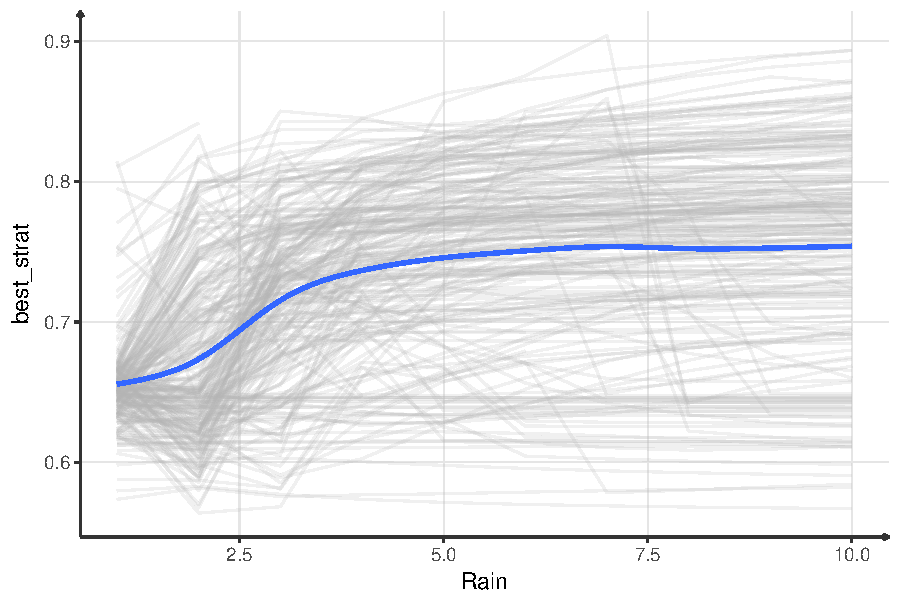
\includegraphics[width = \textwidth]{./Figures/best_strat_rain_gradient.pdf}
\caption{Best strategy for root along a precipitation gradient.}
Growth of plants with different strategies (different RSR and active/structural ratio for roots) along a precipitation gradient have been simulated. The best strat is defined as the weighted mean of the active/structural ratio by the total fresh biomass after 100 days of simulation. Each grey line correspond to a parameter set, while the blue line is the fitted gam regression.
\end{figure}

Equilibrium as major part of plant performance (better perf, even if not best strat, 

%From now memory matters as it defines the phenotypes.

\paragraph{Allocation matters: stability vs risk}
Effect of algo on performance 
$\rightarrow$ why plasticity is important: not only good allocation is important, but also good measure of conditions.\\
\textit{(there is some conceptual drawing to put in here: optimum landscape and how can allocation let you drive in that space.)}\\

Freer allocation algorithms lead to convergence to phenotypes of higher performance. But these phenotype may also be of higher risk ! $\rightarrow $ need for good condition estimation.\\

Importance of having good estimation to have a good strat and good balance.\\

\begin{figure}
\includegraphics[width = \textwidth]{./Figures/max_BM_f_strat_dist.pdf}
\caption{Biomass peak as function of distance to the optimum strategy (a/s ratio)}. Each panel correspond to a precipitation value (not indicated). There is a strong assymetry between more conservative strategies (left) that perform worse but are still viable even far from optimum (positive values far left) and exploitative strategies (right side) that perform well but only if close to the equilibrium. (could it be interesting to show the relationship between strategy and performance variability ?) 

\end{figure}

\paragraph{Plasticity: benefit ?}
Niche experiment = previous analysis discussion. Test hypothesis through simulations for few selected (how ?) parameter sets.\\
Widden niche: 

\subsection{Community level}

Coexisting species ? (look at seed bank to see the traits of coexisting (and persistent) species)
How does plasticity may affect that ?


\section{Discussion}
\paragraph{Individual calibration}
Individual calibration allowed to filter parameters related to individual growth with only few parameters being sensitive.\\

\paragraph{individual growth}
Link memory and phenotype.\\
Link allocation algo and plasticity to the different components of performance.\\
Because the performance depends on multiple aspects of plant allocation in relation with external conditions, it is difficult to isolate each aspect and compute their relative importance or response to certain variables > this is complex to study. Hope this model will help bring more light on plasticity and plant strategies interactions.



\section{Conclusion}
using fundamental "deep" traits and memory: able to reproduce a diversity of resource use strategies. Possibility to \\
%These strategies have an impact on niche and interactions\\
This framework is compatible with phenotypic plasticity\\
plasticity change the niche shape (and probably interactions) and may have an impact on community dynamics.


\section*{References}
\bibliography{../Bibliography/bib_zotero20171106}

\part*{Appendices}

%\section{Theory}

\section{\model description}

\section{State variables, traits and parameters}
\subsection{State variables}
\subsection{Species specific traits}
\subsection{Parameters}

\section{Simulations}


\end{document}